\documentclass[12pt,a4paper]{article}

\usepackage{lips_sve}
\usepackage{natbib}
\usepackage{hyperref}
\usepackage{varioref}
\usepackage{url}
\usepackage{graphicx}
\usepackage{epsfig}
\usepackage{datetime}

%\addto{\captionsswedish}{\renewcommand*{\contentsname}{Table of contents}}
%\addto{\captionsswedish}{\renewcommand*{\tablename}{Table}}

%\newdateformat{\mydate}{\THEDAY - \THEMONTH - \THEYEAR}

%\newcommand{\mytoday}{\formatdate[ddmmyyyy]{\today}}

\begin{document}

\title{Title}
\author{Group 1}
\authorepost{tfya50@googlegroups.com}
\dokument{Final report} \version{0.1}
\filtyp{pdf}
\projektnummer{1} 
\granskad{}{\today}
\godkand{}{\today}
\maketitle
\makestatus
\makeprojektidentitet
\makegruppmedlemmar
\makeprojektinfo
\makeinnehall

\pagenumbering{arabic}
%%%%%%%%%%%%%%%%%%%%%%%%%%%% Introduction %%
\section{Introduction}
\label{sec:Introduction}
This document presents the overview of the project from beginning to end. In this report one can find how the project has worked administratively, what resources were at the group's disposal, what the goal of the product was, how well the goals were reached and how to use the product. The product is an operational Molecular Dynamics (MD) computer program. The end result is a program able to reproduce the real laws of physics at microscopic level so it can be used for realistic predictions in the design of new materials.

%% Involved parties %%
\subsection{Involved parties}
The following parties are involved in this project:
\begin{itemize}
\item the customer
\item the sponsor/course leader
	\begin{itemize}
	\item acts as the customer contact and main project leader
	\item approves the assignment of project leaders
	\item follows the overall execution of the project plan
	\item ultimately validates the outcome and reviews/approves all project documents
	\end{itemize}
\item the project leader
	\begin{itemize}
	\item responsible for the realization of the given tasks and coordination of project members
	\item responsible for respecting and meeting the tollgates/milestones
	\end{itemize}
\item the project members
\item the supervisors/experts
	\begin{itemize}
	\item should be periodically consulted by the project leaders and project members throughout the duration of the project
	\item should expect increased contact in the periods preceding the deadlines for tollgates and milestones
	\end{itemize}
\end{itemize}

%% Project Goal %%
\subsection{Project Goal}
The project goal is to design, implement and operate a Molecular Dynamics (MD) program. Students participating in this project as project members and project leaders should learn the different steps of the MD coding design flow, analyse results obtained with the program and assert the quality of the results. That includes the correct selection and writing of code subroutines, MD program assembling, compiling, debugging and testing, and finally operating the program. 

The project students have an optional choice to add visualization capabilities to the MD code, which would help in understanding and analysing microscopic processes simulated with MD.

%% Usage %%
\subsection{Usage}
The MD program is intended for academic use and it should reliably simulate and calculate materials behaviour and properties. The experience gained in this project could be reused to fully operate and/or develop more complex industrial/academic software used in materials science.

%% Available Resources %%
\subsection{Available Resources}
\begin{itemize}
\item Scientific software
	\begin{itemize}
	\item MD subroutines available (Fortran only). 
	\end{itemize}
\item Scientific publications database
\item Software \& Hardware Tools
	\begin{itemize}
	\item Fortran, C, C++ compilers and related programming software. 
	\item Matlab, Mathematica
	\item Hardware (4 x PCs, running Windows and Linux) \& SUN workstations. 
	\item Dedicated office
	\end{itemize}
\end{itemize}

\newpage
%%%%%%%%%%%%%%%%%%%%%%%%%%%%  Overview of System %%
\section{Overview of Project}
\label{sec:Overview}

%% Project Parts %%
\subsection{Project Parts}
The main parts of the project are:
\begin{itemize}
\item Conceive and design a MD program for a specific class of materials
\item Implement the MD code and test the quality of the MD simulations
\item Operate the MD program to calculate required/additional properties and assess the results
\end{itemize}

%% Project Stages %% 
\subsection{Project Stages}
These are three important stages in this project:
\begin{enumerate}
\item Successful finalisation of the MD computer program
\item Quality assessment of the MD methodology implemented
\item Reliable material properties prediction/calculation, comprehensive analysis of results obtained
\end{enumerate}

%% Education %%
\subsection{Education}
To facilitate the MD program design process, lectures and laboratory exercises were offered before the actual project began.

\newpage
%%%%%%%%%%%%%%%%%%%%%%%%%%%%  Performance and Requirements %%
\section{Performance Requirements}

%% Functionality Requirements %%
\subsection{Functionality Requirements}
Table \ref{tab:Requirements} summarizes the performance requirements of the MD program. Each requirement has a degree of priority is associated.

\begin{table}[h]
\caption{Project requirements with high priority}
\begin{tabular}{| p{0.1\textwidth} | p{0.8\textwidth} | p{0.1\textwidth} |}
	\hline
	Req. 1 & \textbf{MD system set up} atomic configuration, MD parameters, periodic boundary conditions,  neighbour lists etc. & High \\
	\hline
	Req. 2 & \textbf{Interaction potential definition and parameterisation} based on chemical element or material chosen for simulation & High \\
	\hline
	Req. 3 & \textbf{Efficient integrator} for the numerical integration of equations of motion & High \\
	\hline
	Req. 4 & \textbf{Efficient force calculation} analytical or tabulated & High \\
	\hline
	Req. 5 & Routines for calculation of  \textbf{cohesive energy, temperature, internal pressure, thermostat} & High \\
	\hline
	Reg. 6 & \textbf{Capcbility to perform 2-dimensional simulations} necessary for surface properties/processes calculations & High \\
	\hline 
	Req. 7 & \textbf{Visualization capabilities} would be an extremely useful addition and/or upgrade to the MD code & Low \\
	\hline
	Req. 8 & Upgrading with routines allowing the \textbf{calculation of other important material properties} (elastic moduli and constants) & Low \\
	\hline
\end{tabular}
\label{tab:Requirements}
\end{table}

%% Reliability Requirements %%
\subsection{Reliablity Requirements}
Mandatory reliability requirements:
\begin{itemize}
\item all systems simulated using the MD program must correctly reach equilibrium
\item optimize volume of simulated system to have minimal (close to zero) internal pressure
\item correctly estimate the lattice constant of the chosen chemical element/material
\item correctly calculate the cohesive energy of the chemical element/material
\item correctly calculate the mean square displacement (MSD) in 3- and 2-dimensions
\item correctly calculate the diffusion constant for chemical element/material
\item correctly calculate to Debye temperature
\item correctly calculate the specific heat (Cv) of chemical element/material
\end{itemize}

Optional reliability requirements:
\begin{itemize}
\item a number of additional properties, which require the incorporation of more complex routines, can be added to the above list upon the successful completion of the mandatory tasks
\end{itemize}

\newpage
%%%%%%%%%%%%%%%%%%%%%%%%%%%%  Design %%
\section{Design}
The program runs molecular dynamics simulations on several monatomic solids. It uses the Lennard-Jones interaction potential for the interaction between atoms, and the velocity verlet algorithm is used for numerical integration. This section aims to describe in some detail how the program is constructed.

%% Simulation World %%
\subsection{Simulation World}
\label{sec:simulation_world}
The simulation world contains representations of atoms, containing information about position and velocity at a given time, aswell as other nessecery parameters.  All atoms are confined in a section of space, called the bulk, to which is applied periodic boundary conditions to simulate an infinite crystal. The bulk is divided into several smaller regions, called cells, which reduce computation speed. 

\subsubsection{Atoms}
\label{sec:atoms}

\subsubsection{Cells}
\label{sec:cells}
The space of the bulk is divided into a number of cells, all of which span a volume of space. Each cell keeps track of which atoms at a given instant is inside of the cell. The size of a cell is chosen so that all sides of a cell is larger than the potential cutoff distance. This means that an atom only needs to interact with atoms in the same cell and the cells directly next to it. A two dimensional example of the cell structure is shown in figure \ref{fig:cells}. An atom in cell 28 only has neighbors in the nine cells within the marked border. In three dimensions this means that all cells has 27 neighboring cells (itself included). This structure gives a reduced number of atom interactions, disregarding all atom pairs displaced far enough not to give a contribution to the interaction potential. 

\begin{figure}[h]
\begin{center}
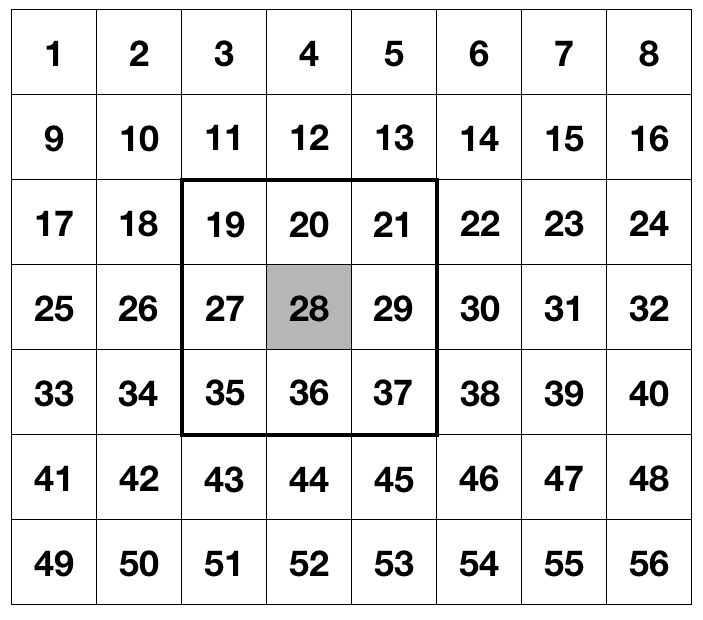
\includegraphics[scale=0.4]{figs/cells.png}
\caption{\small Two-dimensional cell structure
\label{fig:cells}}
\end{center}
\end{figure}

The program uses periodic boundary conditions at the bulk borders. This means that cells which lie on the border of the bulk are in practice in contact with cells on the other side. In the example of figure \ref{fig:cells} the cell number six will be in contact with cells 53, 54 and 55. 


\subsubsection{The periodic boundary condition}
\label{sec:the_periodic_boundary_condition}

\subsubsection{Surface simulations}
\label{sec:surface_simulations}


%% Calculating Physical Properties %%
\subsection{Calculating Physical Properties}
\label{sec:calculating_physical_properties}

%% Graphics %%
\subsection{Graphics}

\newpage
%%%%%%%%%%%%%%%%%%%%%%%%%%%%  Result and discussion %%
\section{Result}
\label{sec:Result}

Total energy plottar för olika lattice constants för att visa att vi hittar den bästa\\
Övriga plottar för den bästa lattice constant (Epot, Ekin, temp, pressure, MSD, Debye, Ecoh, Diffusion coeff, Cv). Plottar finns i appendix B\\
	- Utan termostat\\
	- Med termostat\\
	- Surface utan termostat (ta med de plottar som ser mest vettiga ut)\\
Jämföra dessa plottar och värden med gjorda experiment\\
Visa tabell för vilka material som går att simulera\\
	- Målet: Justera epsilon för alla material\\
	- Visa tabell med alla material, epsilon, Ecoh, diffusion coefficient, Cv\\
Säga att det går att ändra cutoff (ha 8 plottar som visar detta i appendix B)\\
	- Argon, utan termo, 50 K, lattice 1, cutoff 2.5\\
Säga att det går att a icke kubisk bulk (ha 8 plottar som visar detta i appendix B)\\
	- Argon 5x15x12\\
Säga att det går att ändra uppdateringshastigheten för termostaten (ha 8 plottar som visar detta i appendix B)\\
	- Argon, termo, var 500:e steg\\

\newpage

%%%%%%%%%%%%%%%%%%%%%%%%%%%% Appendix A - User Manual %%
\section*{Appendix A - User Manual}

\label{sec:AppendixA}
When the program is run the user will be asked to input certain parameters in order to start the simulation.

\textbf{Start from an old simulation (Yes/No)}: If an old simulation is availible the user can choose to start a new simulation back to back with the old simulation.  

\textbf{Number of unit cells}: Set the number of unit cells in each cartesian direction. The number of cells in each direction does not have to be the same.

\textbf{Periodic boundary condition in z:(Yes/No):} 

\textbf{Time step size:} This determines the time step with which the system progresses. It is given in units of femtoseconds.

\textbf{Number of steps:} Here we choose for how many time steps the simulation will run.

\textbf{Input wanted material:} Choose which material to use in the simulation. The following materials are included in the program and are chosen by inputing their corresponding symbol from the periodic table as follows:

\begin{table}[h]
\begin{center}
\begin{tabular}{l l | l l}
Li & Lithium & Na & Sodium \\
Ar & Argon & K & Potassium \\
Cr & Chromium & Fe & Iron \\
Mo & Molybdenum & W & Wolfram \\
He & Helium & & \\
\end{tabular}
\end{center}
\end{table}


\textbf{Start temperature:} Give the starting temperature for the system in Kelvin.

\textbf{Scaling of lattice constant: }If desired, the lattice constant can be varied in multiples of the pre-set lattice constant for the given material. 

\textbf{Cut-off multiples of the lattice constant:} Sets the cutoff in terms of the the given lattice constant.

\textbf{Simulate with thermostat (Yes/No):} If the temperature of the system is desired, it can be measured if the thermostat is enabled. 

\textbf{Update frequency for the thermostat: }The frequency with which the temperature is measured. \\
After this the simulation is started and the progress is shown each five time steps. \\
When the simulation ends the user is given the specific heat as well as the choice of running another simulation back to back. One is prompted to answer whether or not the system is in equilibrium and then proceed by giving the number of time steps for the continued simulation. 

\textbf{Visualizing the result of the simulation:} 
In order to make the data output from the simulation more clear to the user a Matlab script is provided with the main program. The data from the simulation is automatically exported to a text file which is read by the Matlab script in order to plot how the material properties vary over the time of the simulation. The Matlab script simply needs to be run as is, and the plots will be generated. The properties plotted are total energy, potential energy, kinetic energy, temperature, pressure, mean square displacement, Debye temperature, diffusion coefficient and the cohesive energy.

\newpage
\section{Appendix B - Plots}
\label{sec:AppendixB}
Alla plottar för resultat är här. Kommer hänvisa hit i resultat.


\end{document}
